\documentclass{article}
\linespread{1.3}
\usepackage[margin=50pt]{geometry}
\usepackage{amsmath, amsthm, amssymb, amsthm, tikz, fancyhdr}
\pagestyle{fancy}
\renewcommand{\headrulewidth}{0pt}
\newcommand{\changefont}{\fontsize{15}{15}\selectfont}

\fancypagestyle{firstpageheader}
{
  \fancyhead[R]{\changefont Michael Huang \\ CFRM 415 \\ Midterm}
}

\begin{document}

\thispagestyle{firstpageheader}

\section*{1.}

{\Large 

\subsection*{(a)}

$\mu^T = 
\begin{bmatrix}
  0.3 & 0.6 & 0.7
\end{bmatrix}$ \\
$ \Sigma = 
\begin{bmatrix}
2.5 & 1.2 & 0.3 \\
1.2 & 3.1 & 1.3 \\
0.3 & 1.3 & 2.4
\end{bmatrix}$ \\ 

We optimize by minimizing $\frac{1}{2} \omega^T \Sigma \omega$ with $\omega^T 1 = 1$, and doing the Lagrangian, we find that \\
$\widehat{\omega} = \frac{\Sigma^{-1}1}{1^T\Sigma^{-1}1}$ \\
$\widehat{\omega} = 
\begin{bmatrix}
  0.33604008 \\ 
  0.04578438 \\ 
  0.34986178 \\ 
\end{bmatrix} 
\div
\begin{bmatrix}
  0.73168625
\end{bmatrix}$ \\
$\widehat{\omega} = 
\begin{bmatrix}
  0.459268 \\ 
  0.06257379 \\
  0.47815821
\end{bmatrix}$ \\
The optimal weights are therefore \framebox[1.1\width]{\textbf{0.459268, 0.06257379, 0.47815821}} \\ \\ 
We simply multiply to get the expected annual return: \\
$= \widehat{\omega}^T \cdot  \mu$ \\
$=
\begin{bmatrix}
  0.51003542
\end{bmatrix}$ \\
The expected annual return is therefore \framebox[1.1\width]{\textbf{0.51003542}} \\ \\
To find the portfolio volatility, we find the square root of the variance: \\
$= \sqrt{\widehat{\omega}^T \Sigma \widehat{\omega}}$ \\
$= \sqrt{\frac{1}{1^T \Sigma^{-1} 1}}$ \\
$= \sqrt{1.36670602}$ \\
$= 1.16906203$ \\
The portfolio volatility is therefore \framebox[1.1\width]{\textbf{1.16906203}}

\subsection*{(b)}

Let $\gamma > 0$ be an investor’s risk tolerance. Calculate the mean and variance of the portfolio returns generated by the weights optimizing the general Markowitz optimization problem. Note: You do not need to compute the optimal weights for this case. \\ \\

% Show previous algebra
We define $A = 1^T \Sigma^{-1} 1$, $B = \mu^T \Sigma^{-1} 1$, $C = \mu^T \Sigma^{-1} \mu$. We can calculate these values as scalars, and redefine them as $A = 0.73168625$, $B = 0.3731859$, $C = 0.23130615$.
We know that the portfolio mean can be represented as \\
$\mu = \frac{B}{A} + \frac{1}{\gamma} \frac{AC - B^2}{A}$ \\
$\mu = \frac{0.3731859}{0.73168625} + \frac{1}{\gamma} \frac{0.73168625 \cdot 0.23130615 - 0.3731859^2}{0.73168625}$ \\
$\mu = 0.51003541477 + \frac{1}{\gamma} \frac{0.16924352949 - 0.13926771595}{0.73168625}$ \\
$\mu = 0.51003541477 + \frac{0.04096812471}{\gamma}$ \\
The portfolio mean is therefore \framebox[1.1\width]{\textbf{$0.51003541477 + \frac{0.04096812471}{\gamma}$}} \\ \\
We know that the portfolio variance can be represented as \\
$\sigma^2 = \frac{1}{A} + \frac{1}{\gamma^2} \frac{AC - B^2}{A}$ \\
$\sigma^2 = \frac{1}{0.73168625} + \frac{1}{\gamma^2} \frac{0.73168625 \cdot 0.23130615 - 0.13926771595}{0.73168625}$ \\
$\sigma^2 = 1.36670601641 + \frac{1}{\gamma^2} \frac{0.16924352949 - 0.13926771595}{0.73168625}$ \\
$\sigma^2 = 1.36670601641 + \frac{0.04096812471}{\gamma^2}$ \\
The portfolio variance is therefore \framebox[1.1\width]{\textbf{$1.36670601641 + \frac{0.04096812471}{\gamma^2}$}}

}

\section*{2.}

{\Large

Let $R_i$ and $R_j$ be random variables representing annual excess returns on securities $i$ and $j$ in the total market, under the assumptions of the CAPM. \\

\subsection*{(a)}

By CAPM, we know that \\
$r_i = \alpha_i + r_f + \beta_i(r_M - r_f) + \epsilon_i$ \\ 
$R_i = \alpha_i + \beta_i (r_M - r_f) + \epsilon_i$ \\
\framebox[1.1\width]{\textbf{$R_i = \alpha_i + \beta_i (R_M) + \epsilon_i$}} \\
with $\epsilon_i$ statistically defined with expectation 0, and variance $\sigma_i^2$ \\ \\
We have that $\epsilon_i$ is the idiosyncratic or non-systematic risk since it is directly associated with security $i$, while $\beta_i (R_M)$ is the systematic risk as it is only correlated with the market.
% TODO: Check idiosyncratic

\subsection*{(b)}

We aim to show that $\sigma_{ij} = \beta_i \beta_j \sigma_M^2$, or that $Cov(R_i, R_j) = \beta_i \beta_j \sigma_M^2$. \\
By CAPM, we know that \\
$R_i = \alpha_i + \beta_i (R_M) + \epsilon_i$ \\
$R_j = \alpha_j + \beta_j (R_M) + \epsilon_j$ \\
We can start with $Cov(R_i, R_j)$ \\ 
$= Cov (\alpha_i + \beta_i (R_M) + \epsilon_i, \alpha_j + \beta_j (R_M) + \epsilon_j)$ \\
$= Cov(\beta_i (R_M) + \epsilon_i, \beta_j (R_M) + \epsilon_j)$ \hfill Constants don't affect covariance \\ 
$= Cov(\beta_i (R_M), \epsilon_j) + Cov(\beta_i (R_M), \beta_j (R_M)) + Cov(\beta_j (R_M), \epsilon_i) + Cov(\epsilon_i, \epsilon_j)$ By Hint \\
$= 0 + Cov(\beta_i (R_M), \beta_j (R_M)) + 0 + 0$ \hfill $\epsilon$ is idiosyncratic/specific to security $i/j$ \\ 
$= Cov(\beta_i (R_M), \beta_j (R_M))$ \\
$= \beta_i \beta_j Cov((R_M), (R_M))$ \hfill Definition of covariance \\
$= \beta_i \beta_j Var(R_M)$ \hfill Definition of variance \\
$= \beta_i \beta_j \sigma^2_M$ \\
as we hoped to show.


% As stated previously, by CAPM, we know that $\beta = \frac{Cov(r_p, r_M)}{\sigma_M^2}$

}

\section*{3.}
{\Large 

We are given that $r_f = 0.07, r_M = 0.14, \sigma_M = 0.12$.

\subsection*{(a)}

\begin{figure}[h]
  \centering
  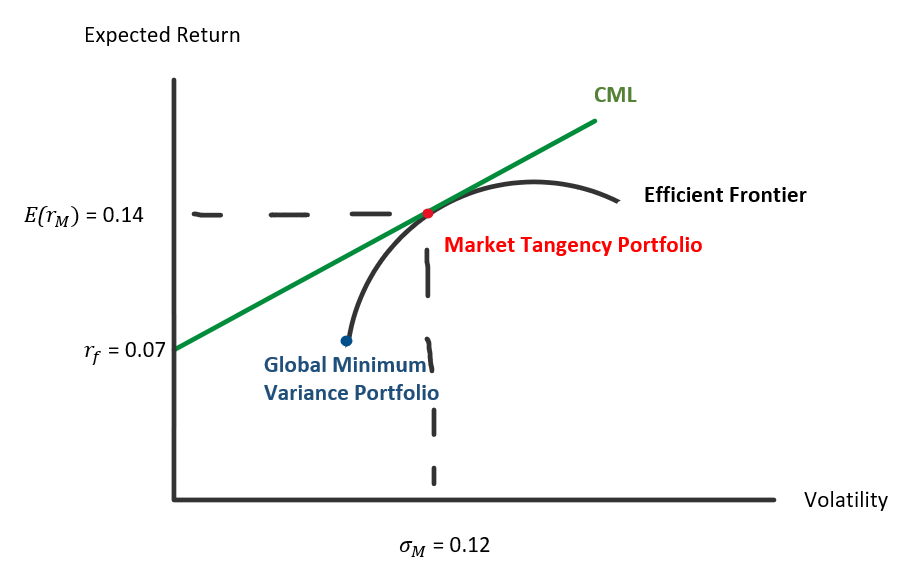
\includegraphics[width=120mm]{./3a.png}
\end{figure}

\subsection*{(b)}

Suppose that of our entire portfolio, we put $y$ towards the market portfolio: \\
$0.11 = 0.07(1-y) + 0.14(y)$ \\ 
$0.11 = 0.07 - 0.07y + 0.14y$ \\ 
$0.04 = 0.07y$ \\ 
\framebox[1.1\width]{\textbf{$y = \frac{4}{7}$ towards the risky asset, and $ 1 - y = \frac{3}{7}$ towards the risk-free asset.}} 


\subsection*{(c)}

We can find the optimal way to invest using the CML which is graphed according to CAPM. A way to do this is by using the equation for the CML. Given two known points (0, 0.07) and (0.12, 0.14), we know its slope to be $\frac{0.14-0.07}{0.12 - 0} = \frac{0.07}{0.12} = \frac{7}{12}$, and the y-intercept to be 0.07. This gives us the equation $0.11 = \frac{7}{12}\sigma + 0.07$. We can therefore solve for the level of volatility for an expected return of 0.11: \\
$0.11 = \frac{7}{12}\sigma + 0.07$ \\
$0.04 = \frac{7}{12}\sigma$ \\
$\frac{1}{25} \cdot \frac{12}{7} = \sigma$ \\
$\frac{12}{175} = \sigma$ \\
$\sigma = $ \framebox[1.1\width]{\textbf{$\sim$ 0.06857}}

}

\section*{4.}
{\Large 

\subsection*{(a)}

\framebox[1.1\width]{\textbf{$T_0 = 2021.05.06$}} \\ 
Count 182 days... \\  
\framebox[1.1\width]{\textbf{$T_1 = 2021.11.06$}} \\
Count 365 days from start... \\
\framebox[1.1\width]{\textbf{$T_2 = 2022.05.06$}}

\subsection*{(b)}

$\tau_1 = \tau(T_0, T_1) = \frac{182 days}{360 days / year} = $ \framebox[1.1\width]{\textbf{0.5055556}} \\
$\tau_2 = \tau(T_1, T_2) = \frac{183 days}{360 days / year} = $ \framebox[1.1\width]{\textbf{0.5083333}} \\
$\tau(T_0, T_2) = \frac{365 days}{360 days / year} = $ \framebox[1.1\width]{\textbf{1.013889}} \\ \\
I used lubridate:
\begin{verbatim}
t0 <- ymd(20210506)
t1 <- ymd(20211104)
t2 <- ymd(20220506)

print(t1 - t0)
print((t1 - t0) / 360)
print(t2 - t1)
print((t2 - t1) / 360)
print(t2 - t0)
print((t2 - t0) / 360)
\end{verbatim}

\subsection*{(c)}

\begin{tabular}{ | c | c | c | c |}
	\hline
		$i$ & $P(T_0, T_i)$ & $P(T_{i-1}, T_i)$ & $L(T_{i-1}, T_i)$ \\
  \hline
		1 & 0.99495720181 & 0.99495720181 & 1\% \\
  \hline
		2 & 0.98490672768 & 0.98989858648 & 2.007\% \\
	\hline
\end{tabular} \\ \\
$P(T_0, T_1) = e^{-R(T_0, T_1)\tau(T_0, T_1)} = e^{-0.01 \cdot 0.5055556} = e^{-0.005055556} = 0.99495720181$ \\
$P(T_0, T_2) = e^{-R(T_0, T_2)\tau(T_0, T_2)} = e^{-0.015 \cdot 1.013889} = e^{-0.015208335} = 0.98490672768$ \\
$P(T_1, T_2) = \frac{P(T_0, T_2)}{P(T_0, T_1)} = \frac{0.98490672768}{0.99495720181} = 0.98989858648$ \\
$L(T_1, T_2) = \frac{1 - P(T_1, T_2)}{\tau(T_1, T_2) P(T_1, T_2)} = \frac{1 - 0.98989858648}{0.5083333 \cdot 0.98989858648}$ = $\frac{0.01010141352}{0.50319841513} = 0.02007441441 = \sim 2.007\%$

\subsection*{(d)}

$S = \frac{\sum_{i=1}^{n} \tau_i P(T_0, T_i) F(T_0; T_{i-1}, T_i)}{\sum_{i=1}^{n} \tau_i P(T_0, T_i)}$ \\
$S = \frac{\tau_1 \cdot P(T_0, T_1) \cdot L(T_0, T_1) + \tau_2 \cdot P(T_0, T_2) \cdot L(T_1, T_2)}{\tau_1 \cdot P(T_0, T_1) + \tau_2 \cdot P(T_0, T_2)}$ \\
$S = \frac{0.5055556 \cdot 0.99495720181 \cdot 0.01 + 0.5083333 \cdot 0.98490672768 \cdot 0.02007}{0.5055556 \cdot 0.99495720181 + 0.5083333 \cdot 0.98490672768}$ \\
$S = \frac{0.01507832585}{1.00366707221}$ \\
\framebox[1.1\width]{\textbf{$S = 0.01502323456$}}

\subsection*{(e)}

To calculate the present value of floating (we start with 1.01 since we just exchanged interest payments): \\
$PV = 1.01 \cdot \sum_{i=1}^{n} \tau_i P(T_0, T_i) F(T_0; T_{i-1}, T_i)$ \\
$PV = 1.01 \cdot \sum_{i=2}^{2} \tau_i P(T_0, T_i) F(T_0; T_{i-1}, T_i)$ \\
$PV = 1.01 \cdot \tau_2 P(T_1, T_2) F(T_1; T_1, T_2)$ \\
$PV = 1.01 \cdot 0.5083333 \cdot  0.98989858648 \cdot 0.02007$ \\
\framebox[1.1\width]{\textbf{$PV = 0.01020018411$}}

\subsection*{(f)}

To calculate the present value of floating with 100,000 (we start with $100,000 \cdot 1.01 = 101,000$ since we just exchanged interest payments): \\
$PV = 101,000 \cdot \sum_{i=1}^{n} \tau_i P(T_0, T_i) F(T_0; T_{i-1}, T_i)$ \\
$PV = 101,000 \cdot \sum_{i=2}^{2} \tau_i P(T_0, T_i) F(T_0; T_{i-1}, T_i)$ \\
$PV = 101,000 \cdot \tau_2 P(T_1, T_2) F(T_1; T_1, T_2)$ \\
$PV = 101,000 \cdot 0.5083333 \cdot 0.98989858648 \cdot 0.02007$ \\
\framebox[1.1\width]{\textbf{$PV = 1020.01841136$}}

}

\section*{5.}
{\Large 

\subsection*{(a)}

Suppose the value of your portfolio is \$1.5 million. Determine the absolute historical Value-at-Risk at 90\% probability, where absolute means to include the mean portfolio return in the result. \\ \\

% Our confidence coefficient is $1 - \alpha = $ 90\%, so we aim to find the z-score for where there is $\alpha = 1 - 0.9 = 0.1$ area under the normal curve to the left. Looking at a table, we can find this to be $\sim -1.28$. \\
% We can calculate the mean and standard deviations of our historical annual data using $\mu = \frac{1}{n} \sum_{i=1}^{n} x_i$ and $\sigma = \sqrt{\frac{1}{n} \sum_{i=1}^{n} (x_i - \mu)^2}$, respectively; we find that $\mu = 0.0565$ and $\sigma = 0.1513$. \\
% Putting this all together, we can take the value at risk at 90\% to be \\
% $|(Z_\alpha\sigma_p + \mu)V_0|$ \\
% $|((-1.28 \cdot 0.1513) + 0.0565) \cdot 1.5\text{+E6}|$ \\
% $|(-0.137164) \cdot 1.5\text{+E6}|$ \\
% $|-205746| = $ \framebox[1.1\width]{\textbf{205746}}
% which means that historically, we have a 90\% probability of losing at most \$205746 in a year (or a 10\% probability of losing more than that in a year).

Our confidence coefficient is $1 - \alpha = 90\%$, so we aim to find the values for the bottom $\alpha = 1 - 0.9 = 0.1$ of all values. Looking at a sorted version of the table, we can see that the bottom $0.10 \cdot 20$ values = 2, and the 2nd-lowest value is $-0.14$. We can also calculate the mean of our historical annual data using $\mu = \frac{1}{n} \sum_{i=1}^{n} x_i$, which we find are $\mu = 0.0565$. \\
We can therefore say that historically, we have a 90\% probability of losing at most \\
$VaR = |(Z_\alpha + \mu)V_0|$ \\
$= |(-0.14 + 0.0565) \cdot 1.5\text{E6}|$ \\
$= |-0.0835 * 1.5\text{E6}| = |-125250|$ \\
$= $ \framebox[1.1\width]{\textbf{125,250}} dollars in a year (or a 10\% probability of losing more than that in a year!).

\subsection*{(b)}

Again, suppose the value of your portfolio is \$1.5 million, and it consists of three funds, with covariance matrix of monthly returns and respective portfolio weights 35\%, 30\%, and 35\%. Compute the relative annual parametric VaR at 95\% probability, assuming normally distributed returns. \\ \\

% $VaR = P \cdot \sigma_P \cdot Z_\alpha$
$\sigma_P^2 = \omega^T \Sigma \omega$ \\
$\sigma_P^2 = 
\begin{bmatrix}
  0.35 & 0.30 & 0.35
\end{bmatrix}
\begin{bmatrix}
  0.25 & 0.12 & 0.03 \\
  0.12 & 0.31 & 0.13 \\
  0.03 & 0.13 & 0.24 \\
\end{bmatrix}
\begin{bmatrix}
  0.35 \\
  0.30 \\
  0.35
\end{bmatrix}$ \\
$\sigma_P^2 = [0.147775]$ \\
$\sigma_P = [0.38441514]$ \\ \\
We know that by definition, since we are using monthly data, annual variance = $12 \sigma_p^2$, so to find annual VaR, we take $-2\sqrt{3}Z_\alpha \sigma_P V_0$. We just found $\sigma_P$. Looking at a z-value table we find that the corresponding z-value for $\alpha = 1 - 0.95 = 0.05$ is approximately $-1.64$. We are given $V_0 = 1.5\text{E6}$. Putting this all together: \\
$\sigma_{PA}^2 = 12 \sigma_p^2$ \\
$VaR_{PA} = |2\sqrt{3} Z_\alpha \sigma_P V_0|$ \\
$VaR_{PA} = |2\sqrt{3} \cdot -1.64 \cdot 0.38441514 \cdot 1.5\text{E6}|$ \\
\framebox[1.1\width]{\textbf{$VaR_{PA} = 3,275,866.64563746$}} 

}


\end{document}